\documentclass[border=10pt]{standalone}
\usepackage{luatexja-fontspec}
\usepackage{tikz}
\usetikzlibrary{positioning, arrows.meta, calc}

% ヒラギノ丸ゴシックを指定
\setmainjfont{HiraMaruProN-W4}

\begin{document}
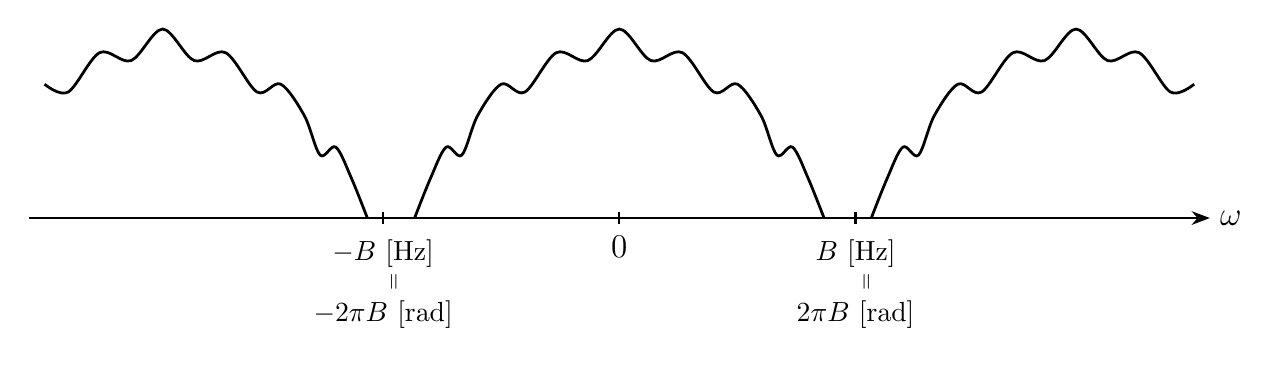
\begin{tikzpicture}[
    thick,                  % 全体の線を太めにする
    >=Stealth,              % 綺麗な矢じりを使用
    font=\large             % フォントサイズを一括で大きくする
]

    % --- 1. 座標軸の描画 ---
    % 周期波形が左右に広がるため、軸の長さを少し広げました（-7.5 から 7.5）
    \draw [->] (-7.5, 0) -- (7.5, 0) node[right] {$\omega$};
    
    % 原点、-B、B の目盛り（小さな縦の区切り線）
    \draw (0, 0.08) -- (0, -0.08);
    \draw (-3, 0.08) -- (-3, -0.08);
    \draw (3, 0.08) -- (3, -0.08);


    % --- 2. スペクトル波形の描画（周期信号） ---
    
    % 【中央の山】（先ほど合意したお気に入りの凸凹波形）
    \draw [black, line width=1.0pt, smooth, tension=0.55] plot coordinates {
        (-2.6, 0.0) (-2.4, 0.5) (-2.2, 0.9) (-2.0, 0.8) (-1.8, 1.3) (-1.5, 1.7)
        (-1.2, 1.6) (-0.8, 2.1) (-0.4, 2.0) (0.0,  2.4) (0.4,  2.0) (0.8,  2.1)
        (1.2,  1.6) (1.5,  1.7) (1.8,  1.3) (2.0,  0.8) (2.2,  0.9) (2.4,  0.5)
        (2.6,  0.0)
    };

    % 【右側の山】（xshiftを使って右へ綺麗に平行移動）
    % 画面外（右端）へ心地よく抜けていくよう、途中の座標まで描画しています
    \begin{scope}[xshift=5.8cm]
        \draw [black, line width=1.0pt, smooth, tension=0.55] plot coordinates {
            (-2.6, 0.0) (-2.4, 0.5) (-2.2, 0.9) (-2.0, 0.8) (-1.8, 1.3) (-1.5, 1.7)
            (-1.2, 1.6) (-0.8, 2.1) (-0.4, 2.0) (0.0,  2.4) (0.4,  2.0) (0.8,  2.1)
            (1.2,  1.6) (1.5,  1.7)
        };
    \end{scope}

    % 【左側の山】（xshiftを使って左へ綺麗に平行移動）
    % 画面外（左端）から入ってくる部分を表現しています
    \begin{scope}[xshift=-5.8cm]
        \draw [black, line width=1.0pt, smooth, tension=0.55] plot coordinates {
            (-1.5,  1.7) (-1.2,  1.6) (-0.8,  2.1) (-0.4,  2.0) (0.0,  2.4)
            (0.4,  2.0) (0.8,  2.1) (1.2,  1.6) (1.5,  1.7) (1.8,  1.3)
            (2.0,  0.8) (2.2,  0.9) (2.4,  0.5) (2.6,  0.0)
        };
    \end{scope}


    % --- 3. 軸下のラベル配置 ---
    % 【原点： 0】
    \node [below=0.1cm of {0, 0}] {$0$};
    
    % 【左側：-B のラベル群】
    \node [below=0.15cm of {-3, 0}, font=\normalsize] (minus_B) {$-B$ [Hz]};
    \node [below=0.05cm of minus_B, font=\normalsize, scale=0.8, rotate=90] {=};
    \node [below=0.15cm of minus_B, font=\normalsize] {$-2\pi B$ [rad]};

    % 【右側：B のラベル群】
    \node [below=0.15cm of {3, 0}, font=\normalsize] (plus_B) {$B$ [Hz]};
    \node [below=0.05cm of plus_B, font=\normalsize, scale=0.8, rotate=90] {=};
    \node [below=0.15cm of plus_B, font=\normalsize] {$2\pi B$ [rad]};

\end{tikzpicture}
\end{document}

